\documentclass[12pt]{article}  

\usepackage
[colorlinks=true, pdfstartview=FitV, linkcolor=blue, citecolor=blue, urlcolor=blue]
{hyperref}

\usepackage{amssymb}  
\usepackage{amsthm}
\usepackage{amsmath}
\usepackage{graphics} 
\usepackage{graphicx} 
%\usepackage[latin1]{inputenc}
\usepackage{tikz}
\usepackage{pgfplots}
\usepackage{wrapfig}
\usepackage{caption}
\usepgfplotslibrary{polar}
\usepackage{ skull }


% GNUPLOT required
\usepackage{verbatim}

\linespread{1.3}

%\addtolength{\textwidth}{80pt}
\addtolength{\evensidemargin}{20pt}
\addtolength{\oddsidemargin}{20pt}

%%%%%%%%%%%%%%%%%%%%%%%%%%%%%%%%%%%%%%%%%%%%%%
%  Begin user defined commands

\newcommand{\map}[1]{\xrightarrow{#1}}

\newcommand{\N}{\mathbb N}
\newcommand{\Z}{\mathbb Z}
\newcommand{\Primes}{\mathbb P}
\newcommand{\Q}{\mathbb Q}
\newcommand{\R}{\mathbb R}
\newcommand{\C}{\mathbb C}
\newcommand{\bz}{\mathbb Z}
\newcommand{\bq}{\mathbb Q}
\newcommand{\br}{\mathbb R}
\newcommand{\bc}{\mathbb C}
\newcommand{\al}{\alpha}
\newcommand{\be}{\beta}
\newcommand{\ga}{\gamma}
\newcommand{\de}{\delta}
\newcommand{\ep}{\epsilon}
\DeclareMathOperator{\lub}{l.u.b.}
%  End user defined commands
%%%%%%%%%%%%%%%%%%%%%%%%%%%%%%%%%%%%%%%%%%%%%%


%%%%%%%%%%%%%%%%%%%%%%%%%%%%%%%%%%%%%%%%%%%%%%
% These establish different environments for stating Theorems, Lemmas, Remarks, etc.

\newtheorem{Thm}{Theorem}
\newtheorem{Prop}[Thm]{Proposition}
\newtheorem{Lem}[Thm]{Lemma}
\newtheorem{Cor}[Thm]{Corollary}

\theoremstyle{definition}
\newtheorem{Def}[Thm]{Definition}

\theoremstyle{remark}
\newtheorem{Rem}[Thm]{Remark}
\newtheorem{Ex}[Thm]{Example}

\theoremstyle{definition}
\newtheorem{Exercise}{Problem}

\newenvironment{Solution}{\noindent\textbf{Solution.}}{}

%\renewcommand{\labelenumi}{(\alph{enumi})}
\renewcommand\qedsymbol{QED}
% End environments 
%%%%%%%%%%%%%%%%%%%%%%%%%%%%%%%%%%%%%%%%%%%%%%%
%Some commands to save paper


\setlength{\parindent}{0in}
\setlength{\parskip}{8pt}

\DeclareMathOperator{\arcsec}{arcsec}
\DeclareMathOperator{\arccot}{arccot}
\DeclareMathOperator{\arccsc}{arccsc}
\DeclareMathOperator{\LH}{\ \underset{\text{LH}}{=}\ }
\newcommand{\Dep}{\Delta_+}
\newcommand{\Dem}{\Delta_-}
\newcommand{\bu}{\mathbf u}
\newcommand{\bv}{\mathbf v}
\newcommand{\bw}{\mathbf w}

\newcommand{\ora}{\overrightarrow}



\addtolength{\textwidth}{80pt}
\addtolength{\evensidemargin}{-40pt}
\addtolength{\oddsidemargin}{-40pt}
\addtolength{\topmargin}{-80pt}
\addtolength{\textheight}{1.8in}

\setlength{\parindent}{0in}
\setlength{\parskip}{8pt}

\DeclareMathOperator{\arcsinh}{arcsinh}

%%%%%%%%%%%%%%%%%%%%%%%%%%%%%%%%%%%%%%%%%%%%%%
% Now we're ready to start
%%%%%%%%%%%%%%%%%%%%%%%%%%%%%%%%%%%%%%%%%%%%%%

\begin{document}  

%\author{Your Name}
{\bf MATH 1103 Homework 2}\\
{\bf Due Friday February 2, 2018}


Practice Problems (not to be turned in)

\vskip5pt
{\bf Practice 1.\ } Use the Geometric Expansion to prove the equality of decimals
\[.99999\dots=1.\]
[Recall that 
$.99999\dots=\lim\limits_{n\to\infty}\left(\dfrac{9}{10}+\dfrac{9}{10^2}+\cdots+\dfrac{9}{10^n}\right).$
]

\begin{Solution}
From the Geometric Expansion we have 
\[\dfrac{9}{10}+\dfrac{9}{10^2}+\cdots+\dfrac{9}{10^n}=
\frac{9}{10}\cdot \frac{1-(9/10)^{n}}{1-(9/10)}\ \to\ 
\frac{9}{10}\cdot \frac{1}{1-(9/10)}=\frac{9}{10-1}=1.
\]

\end{Solution}

{\bf Practice 2.\ }   If humans  had just two fingers, they would express all numbers in binary expansions instead of decimals. Even though they usually have ten fingers,  humans designed computers to express numbers in binary expansions. 

For simplicity, suppose $r$ is a number such that $0<r<1$.
The {\bf binary expansion} of $r$ is 
\[r=.a_1a_2a_3\dots, \]
where each $a_k$ is either $0$ or $1$ and the precise meaning of the expression with $\dots$ is 
\[.a_1a_2a_3\cdots
=\lim_{n\to\infty} \left(\frac{a_1}{2}+\frac{a_2}{2^2}+\cdots+\frac{a_n}{2^n}\right).
\]
For example, the binary expansion of $1/2=.1000\cdots$. 
Just as with decimals, the binary expansion is based on the Geometric Expansion. 

a) Verify the binary expansion
\[\frac{1}{3}= .0101010101\dots
\]

b) Find the binary expansion of $1/13$.

\begin{Solution} 
a)\ The right side is 
\[\lim_{n\to\infty}\left(\frac{1}{4}+\frac{1}{4^2}+\cdots+\frac{1}{4^n}\right)
=\frac{1/4}{1-(1/4)}=\frac{1}{4-1}=\frac{1}{3}.
\]
Note this worked because $3=2^2-1$. If we did not know the binary expansion of $1/3$, we could have found it by doing the above computation in reverse. 

b)\ Before doing $1/13$, let's do $1/7$. This is like part a) becuase $7=2^3-1$. So  we can find the binary expansion of $1/7$ as follows:
\[\frac{1}{7}=\frac{1}{2^3-1}=\frac{(1/2)^3}{1-(1/2)^3}=
\lim_{n\to\infty}\left(\frac{1}{2^3}+\frac{1}{2^6}+\frac{1}{2^9}+\cdots+\frac{1}{2^{3n}}\right)=.001\ 001\ 001\ 001\dots.
\]
Similarly the binary expansion of any number of the form $1/(2^d-1)$, where $d$ is an integer, consists of repeating blocks of $000\cdots 01$ of length $d$. 

Now let's try $1/5$. We have $2^4-1=3\cdot 5$, and $3=2+1$ (which is $11$ in binary), so 
\[\frac{1}{5}=\frac{3}{2^4-1}=\frac{3}{2^4}+\frac{3}{2^{16}}+\frac{3}{2^{64}}+\cdots =.0011\ 0011\ 0011\ \dots.\]

Following this example, here is the recipe for finding the binary expansion of $1/m$ for any odd number $m$. 
\begin{enumerate}
\item Find  the smallest number $d$ such that $m$ divides $2^d-1$ and write $2^{d}-1=a\cdot m$ for some positive integer $a$. 
\item Write $a$ as a sum of descending powers of $2$: 
\[a=2^{d-1}a_1+2^{d-2}a_2+\cdots +2a_{d-1}+a_d,\]
where each of $a_k$ is $0$ or $1$, and $a_d=1$ always. 
\end{enumerate}
Then the binary expansion of $1/m$ is given by  repeating blocks of size $d$:
\[\frac{1}{m}=
.a_1a_2\cdots a_{d}\  \ a_1a_2\cdots a_d\ \ a_1a_2\cdots a_d\ \ 
\dots.
\]
For $m=13$, the smallest $d$ is $d=12$, and 
\[2^{12}-1=(2^6-1)\cdot (2^6+1)=63\cdot 65=315\cdot 13.\]
So $a=315=256+32+16+8+2+1=2^8+2^5+2^4+2^3+2+1$ and we have 
\[
\frac{1}{13}=.000100111011\ 000100111011\ 000100111011\ \dots.
\]
This works with any base which has no divisor in common with $m$.
\end{Solution}

{\bf Practice 3.\ } (Challenging) Prove that a convergent sequence is bounded. 
[Hint: take $\ep=1$ in the definition of convergence, and consider $x_n$ for $n< N$ and $n\geq N$, where $|x-x_n |<1$ for $n\geq N$. ]

\begin{Solution} Since the sequence converges, there is a number $N$ such that $|x-x_n|<1$ for all $n\geq N$. For such $n $ we have 
\[|x_n|=|x_n-x+x|\leq |x-x_n|+|x|\leq 1+|x|.\]
Let $M$ be the largest of the numbers 
$|x_1|,\  |x_2|,\  \dots,\  |x_N|,\  1+|x|$. Then $|x_n|\leq M$ for all $n$.  
\end{Solution}

 \rule{\textwidth}{1pt}
The homework to be turned in may be found on the next page.


\newpage

{\bf Homework to be turned in.}

{\bf 1.\ } A chessboard has 64 squares. Put one grain of rice on the first square, half-a grain of rice on the second square, a fourth of a grain on the third square, an eighth of a grain on the fourth square, and so on for all 64 squares. 
Find the fraction, in lowest terms, of grains of rice on the entire square.  Is this fraction more or less than two grains of rice?

\begin{Solution} 
The total amount of rice is 
\[1+\frac{1}{2}+\frac{1}{4}+\frac{1}{8}+\cdots+\frac{1}{2^{63}}=
\frac{1-(1/2)^{64}}{1-(1/2)}=\frac{2^{64}-1}{2^{63}}=2-\frac{1}{2^{63}}<2.
\]

\end{Solution}

\vskip10pt

{\bf 2.\ } Prove that the sequence $(x_n)$ given by
\[x_n=\frac{1\cdot 3\cdot 5\cdots (2n-1)}{2\cdot 4\cdot 6\cdots (2n)}\]
converges. (You don't have to find the limit.) 

\begin{Solution} We should use a method that does not require knowing the limit. Note that $x_n\geq 0$ and 
\[x_{n+1}=\frac{1\cdot 3\cdot 5\cdots (2n-1)(2n+1)}
{2\cdot 4\cdot 6\cdots (2n)\cdot(2n+2)}=
x_n\cdot \frac{2n+1}{2n+2}<x_n.
\]
So the sequence $(x_n)$ is decreasing, and bounded below by $0$. 
By the Monotone Sequence theorem, $x_n$ converges. 
\end{Solution} 
{\bf comment: } In fact $x_n\to 0$, as we'll see later. 

{\bf 3.\ } Prove that the sequence $(x_n)$ given by
\[x_n=\frac{1}{n+1}+\frac{1}{n+2}+\frac{1}{n+3}+\cdots+\frac{1}{n+n}\]
converges and the limit is somewhere between $0$ and $1$. 


\begin{Solution} Clearly $x_n>0$ and 
\[x_n<\underbrace{\frac{1}{n+1}+\frac{1}{n+1}+\frac{1}{n+1}+\cdots+\frac{1}{n+1}}_{\text{$n$ terms}}=\frac{n}{n+1}<1.
\]
Also, 
\[\begin{split}
x_{n+1}&=\frac{1}{n+1+1}+\frac{1}{n+1+2}+\frac{1}{n+1+3}+\cdots+\frac{1}{n+1+n-1}+\frac{1}{n+1+n}+\frac{1}{n+1+n+1}\\
&=x_n+\frac{1}{n+1+n}+\frac{1}{n+1+n+1}-\frac{1}{n+1}\\
&=x_n+\frac{1}{2n+1}-\frac{1}{2n+2}>x_n,
\end{split}
\]
so the sequence $(x_n)$ is increasing, and is contained in the interval $[0,1]$, so it converges to some number in $[0,1]$. 
\end{Solution} 
{\bf comment: } In fact $x_n\to \log(2)$, as we'll see later. 

More problems on the next page. 
\newpage
\rule{\textwidth}{1pt}
Around the time Isaac Newton was born (1642), Pierre de Fermat (1607-1665, a French judge) determined the area $A$ under the graph of $y=x^p$ above an interval of the form $0\leq x\leq a$, where $p$ is any positive integer (thus improving on Archimedes, who did the case $p=2$, as we saw on the last hw).  Fermat used only the Geometric Series. You will follow Fermat's footsteps in the next few problems. 

Let $r$ be any number such that $0<r<1$, and let $n$ be a positive integer.   
Divide the interval $[0,a]$ into $n+1$ sub-intervals 
\[I_n=[0,ar^n],\quad I_{n-1}=[ar^n,ar^{n-1}],\quad I_{n-2}=[ar^{n-1}, ar^{n-2}],\quad \dots,\quad  I_1=[ar^2,ar],\quad I_0=[ar,a].\]
(See pictures below.)

\rule{\textwidth}{1pt}

{\bf 4.\ } Find the total area of these rectangles below the graph (there is no rectangle above $I_n$) and compute the limit of this area as $n\to\infty$.  Call this limit $L(r)$ ($L$ for ``Lower"). 

\begin{center}
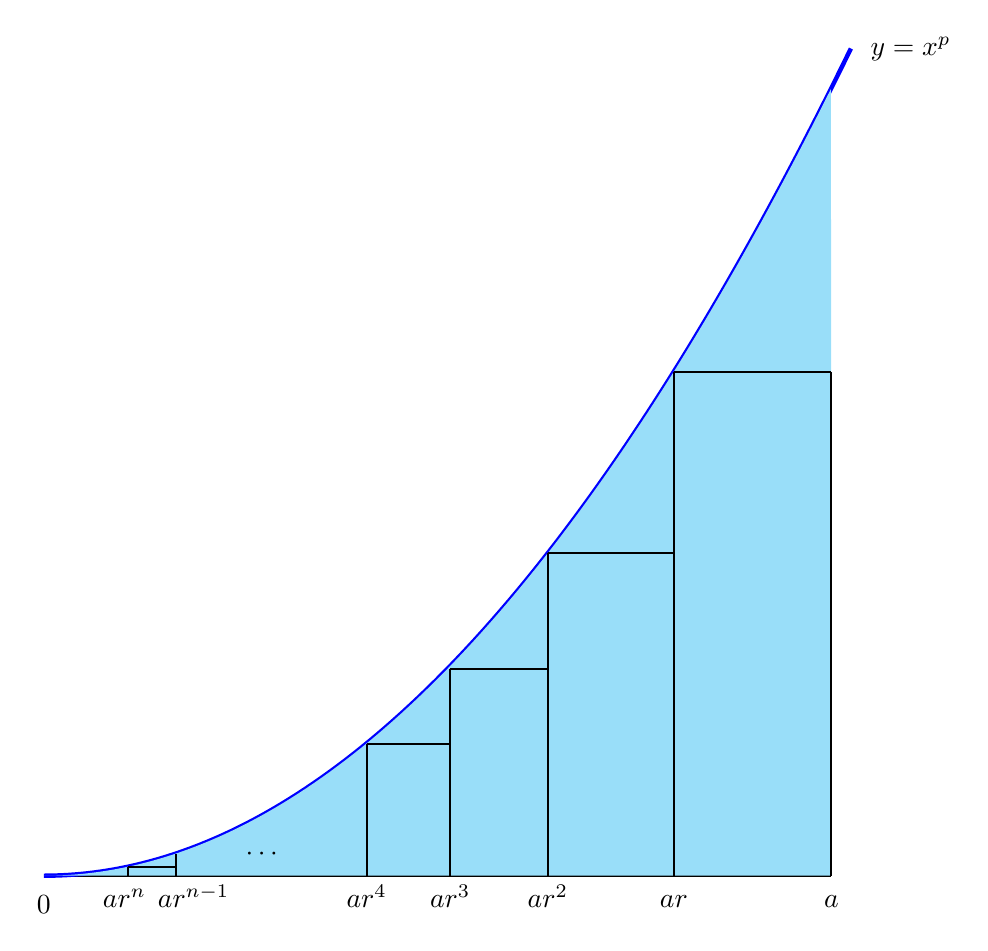
\begin{tikzpicture}[samples=100, domain=0:4, scale=2.5]
\draw[black,   thick] (0,0) -- (4,0 );%a=4
\draw[blue, ultra thick] plot [domain=0: 4.1 ] (\x,{(1/4)*\x*\x)}) ;
\fill[fill=cyan!40!](0,0) -- plot [domain=0:4, ] (\x,{(1/4)*\x*\x)}) -- (4,0) -- cycle;
\draw [black,  thick] (4,0) -- (4,.64*4);

\node[label=right: {$y=x^p$}] at (4.1,4.2) {};
%\node[label=right:
%{$a^{p+1}\cdot \dfrac{r^p}{1+r+\cdots+r^p}\ \leq\ \text{Area}\ \leq \ 
%\dfrac{a^{p+1}}{1+r+\cdots+r^p}$}
%] at (0,3.5) {};

\node[label=below: $0$] at (0,0) {};
\node[label=below: $a$] at (4,0) {};

\node[label=below: $ar$] at (.8*4,0) {}; %r=.8
\draw [black,  thick] (.8*4,0) -- (.8*4,.64*4);
\draw [black,  thick] (.8*4,.64*4) -- (4,.64*4);

\node[label=below: $ar^2$] at (.64*4,0.05) {};
\draw [black,   thick] (.64*4,0) -- (.64*4,.41*4);
\draw [black,  thick] (.64*4,.41*4) -- (.8*4,.41*4);

\node[label=below: $ar^3$] at (.516*4,0.05) {};
\draw [black,  thick] (.516*4,0) -- (.516*4,.2621*4);
\draw [black,  thick] (.516*4,.2621*4) -- (.64*4,.2621*4);

\node[label=below: $ar^4$] at (.41*4,0.05) {};
\draw [black,  thick] (.41*4,0) -- (.41*4,.1677*4);
\draw [black,  thick] (.41*4,.1677*4) -- (.516*4,.1677*4);

\node[label=below: $\cdots$] at (.2621*4+.07,.06*4) {};

\node[label=below: $ar^{n-1}$] at (.1677*4+.09,0.05) {};
\draw [black,  thick] (.1677*4,0) -- (.1677*4,.028*4);
%\draw [black,  thick] (.1073*4,.028*4)-- (.1677*4,.028*4);

\node[label=below: $ar^n$] at (.1073*4-.02,0.03) {};
\draw [black,  thick] (.1073*4,0) -- (.1073*4,.011*4);
\draw [black,  thick] (.1073*4,.011*4) -- (.167*4,.011*4);
%\draw [red,  thick] (.1073*4,.011*4) -- (0,.011*4);
%\draw [red,  thick] (0,0) -- (0,.011*4);
%\draw [red,  thick] (0,0) -- (.1073*4,0);
% 8^3=.512, .8^4=.4096, .8^5=.3277, .8^6=.2621, 
% .8^6=.1677,  .8^10=.1073, .8^12=.0687, .8^14=.044, 
%.8^16=.028, .8^18=.018, .8^20=.011
%
% y=x^2/4
\end{tikzpicture}
\end{center}
\begin{Solution} Starting from the right, the sum of areas (given in width times height) is 
\[\begin{split}(a-ar)\cdot(ar)^p+&(ar-ar^2)\cdot (ar^2)^p+(ar^2-ar^3)\cdot (ar^3)^p+\cdots+(ar^{n-1}-ar^n)\cdot (ar^n)^p\\
&=a^{p+1}(1-r)\left[r^p+r^{2p+1}+r^{3p+2}+\cdots+r^{np+n-1}\right]\\
&=a^{p+1}(1-r)r^p\left[1+r^{p+1}+\left(r^{p+1}\right)^2+\cdots+
\left(r^{p+1}\right)^{n-1}\right]\\
&=a^{p+1}(1-r)r^p\cdot\frac{1-\left(r^{p+1}\right)^n}{1-r^{p+1}}.
\end{split}
\]
Taking the limit as $n\to \infty$ we get (since $0<r^{p+1}<1$) 
\[
L(r)=a^{p+1}(1-r)r^p\cdot\frac{1}{1-r^{p+1}}=
\frac{a^{p+1}r^p}{1+r+r^2+\cdots +r^p}.
\]


\end{Solution}


{\bf 5.\ } Find the total area of these rectangles above the graph (including the little red rectangle above $I_n$) and take the limit of this area as $n\to\infty$. Call this limit $U(r)$ ($U$ for ``Upper").

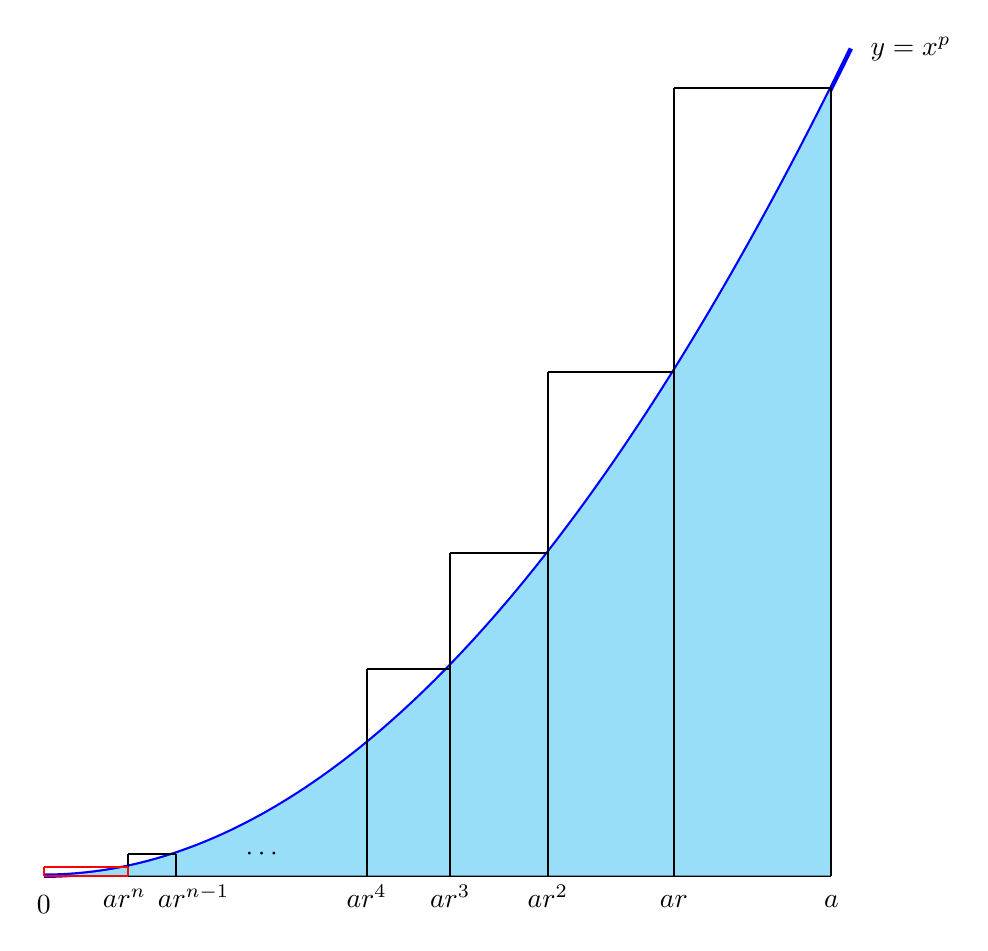
\begin{tikzpicture}[samples=100, domain=0:4, scale=2.5]
\draw[black,   thick] (0.073*4,0) -- (4,0 );%a=4
\draw[blue, ultra thick] plot [domain=0: 4.1 ] (\x,{(1/4)*\x*\x)}) ;
\fill[fill=cyan!40!](0,0) -- plot [domain=0:4, ] (\x,{(1/4)*\x*\x)}) -- (4,0) -- cycle;
\draw [black,  thick] (4,0) -- (4,4);

\node[label=right: {$y=x^p$}] at (4.1,4.2) {};

\node[label=below: $0$] at (0,0) {};
\node[label=below: $a$] at (4,0) {};

\node[label=below: $ar$] at (.8*4,0) {}; %r=.8
\draw [black,  thick] (.8*4,0) -- (.8*4,4);
\draw [black,  thick] (.8*4,4) -- (4,4);

\node[label=below: $ar^2$] at (.64*4,0.05) {};
\draw [black,   thick] (.64*4,0) -- (.64*4,.64*4);
\draw [black,  thick] (.64*4,.64*4) -- (.8*4,.64*4);

\node[label=below: $ar^3$] at (.516*4,0.05) {};
\draw [black,  thick] (.516*4,0) -- (.516*4,.4096*4);
\draw [black,  thick] (.516*4,.4096*4) -- (.64*4,.4096*4);

\node[label=below: $ar^4$] at (.41*4,0.05) {};
\draw [black,  thick] (.41*4,0) -- (.41*4,.2621*4);
\draw [black,  thick] (.41*4,.2621*4) -- (.516*4,.2621*4);

\node[label=below: $\cdots$] at (.2621*4+.07,.06*4) {};

\node[label=below: $ar^{n-1}$] at (.1677*4+.09,0.05) {};
\draw [black,  thick] (.1677*4,0) -- (.1677*4,.028*4);
\draw [black,  thick] (.1073*4,.028*4)-- (.1677*4,.028*4);

\node[label=below: $ar^n$] at (.1073*4-.02,0.03) {};
\draw [black,  thick] (.1073*4,0) -- (.1073*4,.028*4);
\draw [red,  thick] (.1073*4,0) -- (.1073*4,.011*4);
\draw [red,  thick] (.1073*4,.011*4) -- (0,.011*4);
\draw [red,  thick] (0,0) -- (0,.011*4);
\draw [red,  thick] (0,0) -- (.1073*4,0);
% 8^3=.512, .8^4=.4096, .8^5=.3277, .8^6=.2621, 
% .8^6=.1677,  .8^10=.1073, .8^12=.0687, .8^14=.044, 
%.8^16=.028, .8^18=.018, .8^20=.011
%
% y=x^2/4
\end{tikzpicture}

\begin{Solution} Starting from the right, the sum of areas  is 
\[\begin{split}(a-ar)\cdot a^p+&(ar-ar^2)\cdot (ar)^p+(ar^2-ar^3)\cdot (ar^2)^p+\cdots+(ar^{n-1}-ar^n)\cdot (ar^{n-1})^p
+ar^n\cdot(ar^n)^p\\
&=a^{p+1}(1-r)\left[1+r^{p+1}+r^{2p+2}+r^{3p+3}+\cdots+r^{(n-1)(p+1)}\right]+(ar^n)^{p+1}\\
&=a^{p+1}(1-r)\left[1+r^{p+1}+\left(r^{p+1}\right)^2+\left(r^{p+1}\right)^3+\cdots+
\left(r^{p+1}\right)^{n-1}\right]+a^{p+1}\left(r^{p+1}\right)^n\\
&=a^{p+1}(1-r)\cdot\frac{1-\left(r^{p+1}\right)^n}{1-r^{p+1}}
+a^{p+1}\left(r^{p+1}\right)^n.
\end{split}
\]
Taking the limit as $n\to \infty$ we get (again, since $0<r^{p+1}<1$) 
\[
U(r)=a^{p+1}(1-r)\cdot\frac{1}{1-r^{p+1}}=
\frac{a^{p+1}}{1+r+r^2+\cdots +r^p}.
\]

\end{Solution}

{\bf 6.\ } From the pictures, we have $L(r)<A<U(r)$.  Compute the limits of $L(r)$ and $U(r)$ as $r\to 1$ and 
thereby compute $A$ as Fermat did. 
\vskip5pt
\begin{Solution} From 4 and 5 we have 
\[\frac{a^{p+1}r^p}{1+r+r^2+\cdots +r^p}\ < \ A\ <\ 
\frac{a^{p+1}}{1+r+r^2+\cdots +r^p}.
\]
Taking the limit as $r\to1$, the outer two terms go to
\[\frac{a^{p+1}}{1+1+1^2+\cdots +1^p}=\frac{a^{p+1}}{p+1}.\]
By the Squeeze Law, Fermat (and we) have shown that 
\[A=\frac{a^{p+1}}{p+1}.\]

\end{Solution}

{\bf comment:\ } Using the language of Quadrature, Fermat would have said the area $A$ is equal to the area of the rectangle on the same base, with height equal to $1/(p+1)$ of the height of the region under the graph. 
If $p=1$ this region is just a triangle and we get the familiar formula Area=$1/2$-base-times-height. If $p=2$ the result $a^3/3$ is equivalent to Archimedes' formula. 

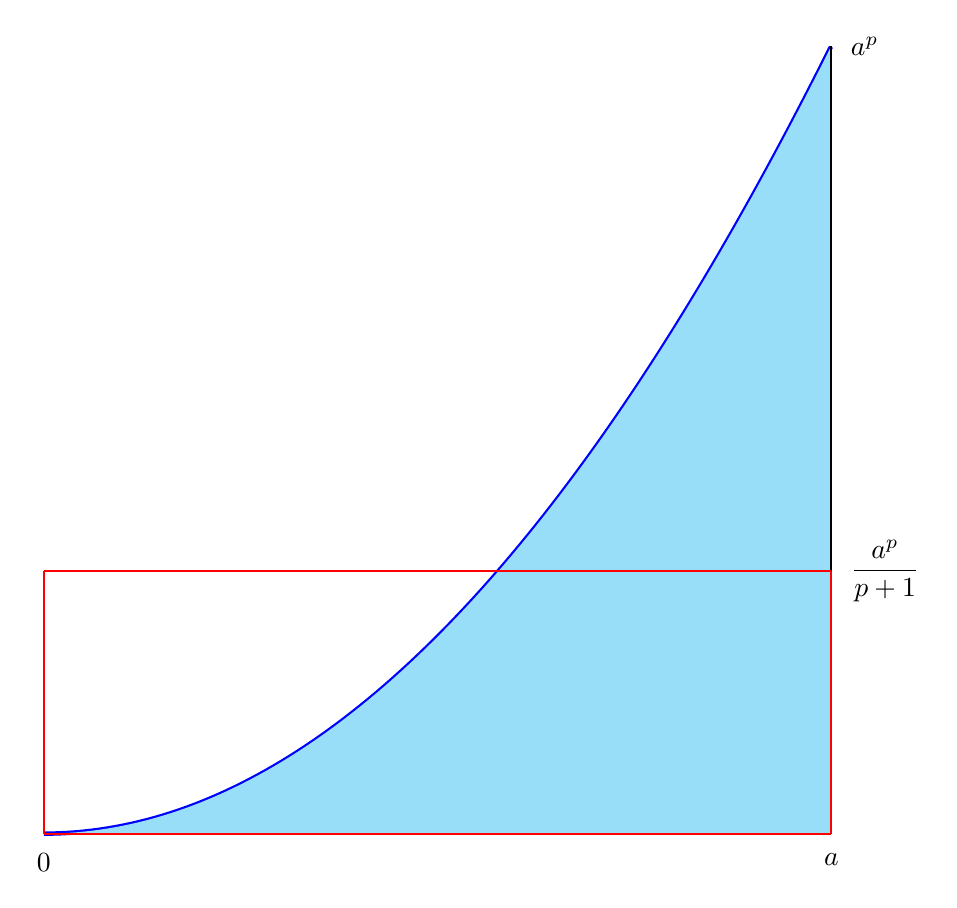
\begin{tikzpicture}[samples=100, domain=0:4, scale=2.5]
\draw[black,   thick] (0.073*4,0) -- (4,0 );%a=4
\draw[blue, ultra thick] plot [domain=0: 4 ] (\x,{(1/4)*\x*\x)}) ;
\fill[fill=cyan!40!](0,0) -- plot [domain=0:4, ] (\x,{(1/4)*\x*\x)}) -- (4,0) -- cycle;
\draw [black,  thick] (4,0) -- (4,4);
\draw [red,  thick] (4,0) -- (4,4/3);
\draw [red,  thick] (4,4/3) -- (0,4/3);
\draw [red,  thick] (0,4/3) -- (0,0);
\draw [red,  thick] (0,0) -- (4,0);
%\node[label=above: {$y=x^p$}] at (4.1,4.2) {};
\node[label=right: $a^p$] at (4,4) {};
\node[label=right: $\dfrac{a^p}{p+1}$] at (4,4/3) {};
\node[label=below: $0$] at (0,0) {};
\node[label=below: $a$] at (4,0) {};

% y=x^2/4
\end{tikzpicture}

\end{document}

 
 
